\chapter{AĞ GÜVENLİĞİ MİMARİSİ VE ALTYAPI KORUMA}

\section*{Giriş}
Bu kapsamlı eğitim belgesi, siber güvenlik alanındaki uzmanlar için tasarlanmıştır ve modern ağ güvenliği mimarilerinin temelini oluşturan prensipleri, teknolojileri ve pratik uygulamaları detaylandırmaktadır. Bu bölüm, ağ altyapısının korunması için hem teorik hem de uygulamalı bir çerçeve sunmaktadır.

\section{Ağ Güvenlik Mimarisi ve Tasarım Prensipleri}

Modern ağ güvenliği, tek bir savunma hattına dayanmaktan ziyade, stratejik olarak katmanlanmış ve birbirini tamamlayan mekanizmalarla oluşturulan sağlam bir mimariyi gerektirir. Bu yaklaşım, bir siber saldırganın ağa erişimini zorlaştırmak, ihlalin etki alanını sınırlamak ve tespit edilme şansını artırmak için tasarlanmıştır.

\subsection{Defense-in-Depth Network Architecture (Katmanlı Savunma Ağ Mimarisi)}

Defense-in-Depth (DiD), bir bilgi güvenliği felsefesidir ve bir ağdaki gizlilik, bütünlük ve erişilebilirliği korumak için bir dizi güvenlik mekanizmasının ve kontrolünün katmanlar halinde yerleştirilmesini ifade eder. Hiçbir bireysel önlem tüm siber tehditleri durduramaz, ancak birlikte çalışarak çok çeşitli tehdit vektörlerine karşı koruma sağlarlar ve bir mekanizma başarısız olduğunda yedeklilik sunarlar. Bu strateji başarılı olduğunda, ağın güvenliğini birçok farklı saldırı vektörüne karşı önemli ölçüde güçlendirir.
Bu katmanlı yaklaşım, bir ağda birden fazla güvenlik kontrolünün stratejik olarak konumlandırılmasını içerir. Bu katmanlar, geleneksel ağ güvenlik duvarlarından (firewalls), kötü niyetli trafiği tespit edip engelleyen Saldırı Tespit ve Önleme Sistemlerine (IDS/IPS) kadar uzanır. Ayrıca, kullanıcıların dizüstü bilgisayarları veya mobil cihazları gibi uç noktalara yerleştirilen antivirüs koruması, tehdit tespiti ve analizi sağlayan Uç Nokta Tespit ve Yanıt (EDR) yazılımlarını da kapsar. Temel bir adım olan ağ segmentasyonu, ağı iş ihtiyaçlarına göre alt ağlara ayırarak yanal hareketin önlenmesine yardımcı olurken, Çok Faktörlü Kimlik Doğrulama (MFA) ve şifreleme gibi önlemler, kullanıcı ve veri düzeyinde koruma sağlar.
Bu güvenlik felsefesinin altında yatan temel mantık, siber güvenlikte "tek bir gümüş kurşun"un olmadığıdır. Bir saldırgan, bir katmanı aşsa bile, bir sonraki katmanla karşılaşır. Bu durum, başarılı bir ağ ihlali için gereken süreyi ve karmaşıklığı artırır, böylece aktif bir saldırının tamamlanmadan önce tespit edilme ve durdurulma olasılığını yükseltir. Bu katmanlı savunma yaklaşımı, fiziksel güvenlikte de rutin olarak uygulanmaktadır. Örneğin, değerli varlıkları korumak için güvenlik kameraları, kurşun geçirmez cam ve kasaların kullanılması, aynı prensibin somut bir örneğidir. Bu paralellik, siber güvenlik uzmanlarının hem dijital hem de fiziksel güvenlik problemlerinin temelinde yatan ortak mantığı anlaması gerektiğini göstermektedir. Bir ağın savunmasını, bir kalenin kapıları, duvarları ve hendekleri gibi katman katman korumaya benzetmek, sadece bir ağa rastgele güvenlik araçları eklemekten daha fazlası olduğunu, bir güvenlik mimarisi oluşturma yaklaşımı olduğunu vurgular.

\subsection{Network Segmentation ve Micro-segmentation Stratejileri}

Ağ segmentasyonu, bir ağı daha küçük, izole edilmiş segmentlere ayırma uygulamasıdır ve siber güvenlik riskini azaltmanın hayati bir adımıdır. Mikro-segmentasyon ise bu yaklaşımın daha granüler bir formudur; ağı iş yükleri, uygulamalar ve hatta bireysel cihazlar düzeyinde izole eder. Bu strateji, bir saldırganın ağa ilk erişimi sağladıktan sonra yanal hareketini (lateral movement) zorlaştırarak bir ihlalin etki alanını ("blast radius") sınırlar ve genel saldırı yüzeyini azaltır.
Bu stratejiyi başarılı bir şekilde uygulamak, metodolojik bir süreç gerektirir:

\begin{enumerate}
\item \textbf{Değerli Veri ve Varlıkları Tanımlama:} Bir kuruluştaki tüm veri ve varlıklar aynı değere sahip değildir. Müşteri veritabanı gibi operasyonlar için hayati olan sistemlerin belirlenmesi ilk adımdır.
\item \textbf{Sınıflandırma Etiketleri Atama:} Hassasiyet seviyelerine göre varlıklara etiketler atayın (örneğin, "Gizli," "Özel"). Bu etiketler, daha sonra ağ içindeki güven bölgelerini tanımlamak için kullanılır.
\item \textbf{Veri Akışlarını Haritalama:} Ağ genelindeki veri akışlarını haritalayarak uygulamalar ve sistemler arasındaki iletişim ve bağımlılıkları belirleyin. Bu, segmentasyon politikalarının oluşturulması için temel bir adımdır.
\item \textbf{Varlık Grupları Tanımlama:} Benzer amaçlara ve hassasiyet seviyelerine sahip varlıkları ayrı segmentlerde gruplandırın.
\item \textbf{Erişim Kontrol Politikaları Oluşturma:} En az ayrıcalık prensibine dayalı olarak segmentler arası iletişimi düzenleyen politikalar oluşturun. Bu, bir uygulamanın veya kullanıcının işini yapmak için gerekli olan minimum izin seviyesine sahip olmasını sağlar.
\end{enumerate}

Ağ segmentasyonu, sadece bir saldırı kontrolü değildir; aynı zamanda bir \textbf{Sıfır Güven (Zero Trust) modelinin teknik temelidir}. Sıfır Güven, ağ içinde hiçbir şeye varsayılan olarak güvenmemeyi gerektirir. Bir ağ, mantıksal olarak izole edilmiş segmentlere ayrıldığında, her bir segment sınırı, bu "hiçbir şeye güvenme" politikasının uygulanabileceği bir kontrol noktası haline gelir. Bu, teorik bir modelin pratik bir mimariye dönüşmesini sağlayan kritik bir adımdır.

\subsection{Zero Trust Network Architecture (ZTNA) Modeli}

Zero Trust Network Architecture (ZTNA), geleneksel güvenlik modellerinden önemli bir sapma gösteren bir yaklaşımdır. Bu model, bir ağda herhangi bir iç veya dış kullanıcıya ya da cihaza varsayılan olarak güvenmek yerine, her erişim isteğini sürekli olarak doğrular ve yetkilendirir. Geleneksel güvenlik, ağ çevresini bir kale gibi savunurken, ZTNA bir ihlalin zaten meydana geldiğini varsayar ("assume a breach") ve güveni ağın her noktasına yerleştirir.

\begin{figure}[H]
    \centering
    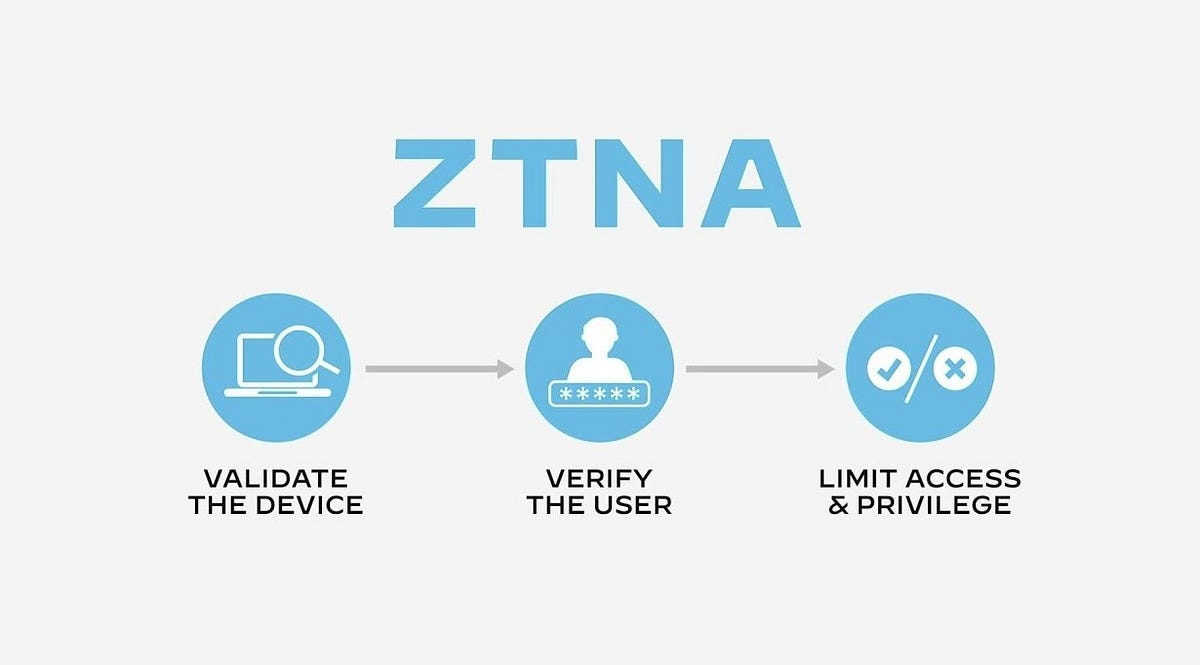
\includegraphics[width=0.8\textwidth]{img/ZTNA.png}
    \caption{Sıfır Güven (Zero Trust) Ağ Erişim Mimarisi}
    \label{fig:ztna}
\end{figure}
ZTNA, geleneksel VPN'lerden farklı olarak, kimlik doğrulamayı kullanıcının IP adresine değil, daha gelişmiş kimlik tekniklerine dayandırır. Bu, kuruluşa, kullanıcı konumuna veya cihaz türüne göre erişim isteklerini otomatik olarak reddetme gibi özelleştirilmiş ve granüler güvenlik politikaları oluşturma esnekliği sunar. Bir kullanıcının kimliği bir kez doğrulandıktan sonra tüm ağa erişim sağlayan VPN'lerin aksine, ZTNA en az ayrıcalık prensibini uygulayarak yalnızca kullanıcının ihtiyaç duyduğu uygulamalara ve hizmetlere erişim sağlar.
Bir ZTNA modelini uygulamak, teknolojik araçlardan daha fazlasını gerektiren metodolojik bir süreçtir. Aşağıdaki beş adım, Zero Trust yaklaşımını uygulamak için yaygın olarak kullanılan bir kılavuzdur:

\begin{enumerate}
\item \textbf{Koruma Yüzeyini Tanımlama:} Saldırı yüzeyini tanımlayın ve en değerli dijital varlıklara (hassas veriler, kritik uygulamalar ve hizmetler) odaklanın.
\item \textbf{Ağ Kontrolleri Uygulama:} Ağınızdaki trafik akışını ve sistem bağımlılıklarını anlayın.
\item \textbf{Bir Sıfır Güven Ağı Mimarisi Oluşturma:} Ağ segmentasyonunu uygulayın ve çok faktörlü kimlik doğrulamayı (MFA) dahil edin.
\item \textbf{Bir Sıfır Güven Politikası Oluşturma:} Her bir erişim isteği için "Kim, Ne, Ne Zaman, Nerede, Neden ve Nasıl" (Kipling Metodu) sorularını sorarak politikalar tasarlayın.
\item \textbf{Ağı İzleme:} Potansiyel sorunları daha erken tespit etmek için ağ aktivitesini sürekli olarak izleyin; bunun için raporlar, analizler ve loglar kullanılır.
\end{enumerate}

ZTNA'nın uygulanması, organizasyonel bir zihniyet değişikliği ve paydaş katılımı gerektiren kaynak yoğun bir süreçtir. Bu, güvenlik politikalarını otomatikleştirme ve sürekli doğrulama için gerekli süreç ve araçları yeniden tasarlamayı içerir. ZTNA, bir teknoloji satın almaktan ibaret değildir; bu, bir kuruluşun güvenliğe yaklaşımını baştan aşağı yeniden tanımlayan stratejik bir operasyonel yeniden yapılanmadır.

\subsection{Software-Defined Perimeter (SDP) Yaklaşımları}

Software-Defined Perimeter (SDP), ağ altyapısını internete karşı görünmez hale getirerek, DDoS, fidye yazılımı ve sunucu taraması gibi ağ tabanlı saldırılara karşı savunmasızlığı azaltan bir yaklaşımdır. SDP, bir kullanıcının kimliğini ve cihaz duruşunu doğrulayarak kaynaklara sanal bir sınır oluşturur ve yalnızca yetkili kullanıcıların erişimini sağlar. Bu yöntem, bir Zero Trust güvenlik modelini uygulamak için kritik bir rol oynar.
SDP, geleneksel Sanal Özel Ağlara (VPN) göre önemli avantajlar sunar. Geleneksel VPN'ler, kullanıcılara ağa tam erişim sağlarken, SDP'ler özelleştirilmiş politikalara dayalı olarak yalnızca uygulamalara ve hizmetlere erişim sağlar. Bu, bir kullanıcının bir ağ varlığına erişimi olmaması durumunda onu görmesini de engeller. Ayrıca, SDP her kullanıcı için ayrı ve şifreli bir ağ bağlantısı oluşturarak bir saldırganın ağ içinde serbestçe dolaşma (roam) yeteneğini sınırlar. SDP, Zero Trust'ın "karanlık bulut" (dark cloud) konseptini hayata geçirir; yani kullanıcılar, izinleri olmayan uygulama ve hizmetleri göremezler. Bu, potansiyel bir saldırganın ağdaki kaynakları taramasını ve yanal hareket etmesini önleyerek saldırı yüzeyini önemli ölçüde azaltır.
SDP, esnek, tutarlı ve merkezi politika yönetimi sağlar. Geleneksel sistemlerin aksine, SDP politikaları otomasyonu destekler, bu da dinamik BT ortamlarında ölçeklenebilirlik sağlar. Bu teknoloji, dizüstü bilgisayarlar, mobil cihazlar ve IoT aygıtları dahil olmak üzere geniş bir cihaz yelpazesini destekler. Özünde, SDP, geleneksel ağ merkezli (network-centric) VPN'lerden farklı olarak kimlik ve uygulama merkezli (identity- and application-centric) bir model sunar. Bu, onu modern, dağıtık ve bulut tabanlı çalışma ortamları için tasarlanmış, doğası gereği bir ZTNA platformu yapar.

\subsection{DMZ (Demilitarized Zone) Tasarımı ve Best Practices}

Demilitarized Zone (DMZ), bir kuruluşun yerel ağı (LAN) ile halka açık internet arasında ek bir güvenlik katmanı olarak işlev gören bir alt ağdır. DMZ, web sunucuları, e-posta sunucuları ve DNS sunucuları gibi, dış kullanıcıların erişmesi gereken, dışa dönük hizmetleri barındırır. Bu yapılandırmanın amacı, bu hizmetler ihlal edilse bile, saldırganın ana iç ağa doğrudan erişimini engellemektir.
DMZ'yi tasarlamak için kullanılan iki ana mimari model bulunmaktadır:

\begin{itemize}
\item \textbf{Tek Güvenlik Duvarı (Üç Ayaklı Model):} En az üç ağ arayüzüne sahip tek bir güvenlik duvarı kullanılır. Bir arayüz dış ağa, bir arayüz iç ağa ve bir arayüz DMZ'ye bağlanır. Bu yapı, basitlik sağlar, ancak DMZ'deki bir ihlal durumunda iç ağın doğrudan korunması için ek bir güvenlik duvarı kadar sağlam olmayabilir.
\item \textbf{Çift Güvenlik Duvarı Mimarisi:} İki ayrı güvenlik duvarı kullanılır. Birincisi, dış ağ ile DMZ arasında bir "ön uç" güvenlik duvarı olarak işlev görür ve yalnızca DMZ'ye yönelik trafiğe izin verir. İkincisi, DMZ ile iç ağ arasında "arka uç" güvenlik duvarı olarak çalışır ve yalnızca DMZ içindeki onaylanmış kaynaklardan gelen trafiğe izin verir. Bu daha güvenli bir yaklaşımdır ve hassas kaynakları barındıran kuruluşlar için tavsiye edilir.
\end{itemize}

DMZ'nin etkinliği, güvenlik duvarı kurallarının doğru bir şekilde uygulanmasına bağlıdır. İşte en iyi uygulamalardan bazıları:

\begin{itemize}
\item \textbf{Sıkı Güvenlik Duvarı Kuralları:} Dış güvenlik duvarı, yalnızca web sunucuları için TCP 80 ve 443 gibi belirli hizmet portlarına izin verecek şekilde yapılandırılmalıdır. Tüm diğer istekler engellenmelidir. İç güvenlik duvarı kuralları daha katı olmalıdır; yalnızca DMZ'deki onaylanmış kaynaklardan gelen trafiğe iç ağa erişim izni verilmelidir.
\item \textbf{Ağ Adres Çevirisi (NAT):} Özel IP adreslerinin ve yönlendirme bilgilerinin yetkisiz kişilere ifşa edilmemesi için NAT'ı kullanın.
\item \textbf{Düzenli Denetim:} DMZ'yi ve güvenlik duvarı kurallarını, amaçlandığı gibi çalıştıklarından emin olmak için düzenli olarak test edin ve denetleyin. Gereksiz, güncel olmayan veya yanlış kuralları temizleyin.
\end{itemize}

DMZ tasarımı, basit bir araç uygulamasından daha fazlasıdır; risk toleransına ve iş mantığına dayalı bir mimari kararıdır. Bir siber güvenlik uzmanı, bir DMZ'nin nasıl tasarlanacağını seçerken, kuruluşun barındırılan hizmetlerin hassasiyetine ve potansiyel bir ihlalin riskine dayalı olarak güvenlik ve karmaşıklık arasındaki dengeyi anlamalıdır.

\section{Next-Generation Firewall (NGFW) ve Güvenlik Duvarları}

Next-Generation Firewalls (NGFW), geleneksel güvenlik duvarlarının ötesine geçerek gelişmiş özellikler sunan üçüncü nesil güvenlik duvarı teknolojisidir. NGFW'ler, paket filtreleme ve durum bilgili denetim gibi temel yetenekleri, uygulama seviyesinde tehditleri ele alan akıllı ve bağlam odaklı güvenlik özellikleriyle birleştirir. Bu, modern siber tehditlere karşı daha kapsamlı bir koruma sağlar.

\subsection{Stateful Packet Inspection vs Deep Packet Inspection}

Geleneksel güvenlik duvarı teknolojisinin temelinde durum bilgili paket denetimi (Stateful Packet Inspection) bulunur. Bu yöntem, bir paketin yalnızca başlık bilgisini (kaynak/hedef IP adresi ve port numarası gibi) kontrol ederek ağ trafiğini kontrol eder. Bu, bir bağlantıdaki tüm paketlerin durumunu izleyerek trafik akışlarını daha etkili bir şekilde yönetir. Ancak, bu yaklaşım, paketin içeriğini incelemediği için başlık bilgilerini gizleyebilecek tehditlere karşı savunmasız kalır.
Derin paket denetimi (Deep Packet Inspection - DPI), bu sınırlamanın üstesinden gelir. DPI, bir paketin başlığının yanı sıra taşıdığı verinin tamamını da inceler. Bu sayede, geleneksel filtreleme yöntemlerinin gözden kaçırabileceği, veri sızdırma girişimleri, içerik politikası ihlalleri veya zararlı yazılımlar gibi gizli tehditleri bulabilir. DPI, aynı zamanda, daha yüksek öncelikli trafiğe (VoIP veya Zoom gibi) öncelik vermek için de kullanılabilir.
Ancak, DPI'nin bu gelişmiş güvenliği, bazı ödünleşmelerle birlikte gelir. DPI, ağ trafiği üzerinde büyük bir işlem yükü oluşturur, bu da ağ hızını ve performansını düşürebilir. Ayrıca, mevcut güvenlik duvarlarının karmaşıklığını artırır ve optimum etkinlik için periyodik güncellemeler ve revizyonlar gerektirir. Bu, siber güvenlikte "güvenlik, performans ve kullanılabilirlik" arasındaki temel bir ödünleşimi gösterir. Bir siber güvenlik uzmanı, DPI'nin sağladığı güvenlik faydalarını operasyonel maliyetlerinden ayrı düşünemez.

\subsection{Application-aware Firewalling ve Layer 7 Security}

OSI modelinin en üst seviyesi olan Layer 7 (Uygulama Katmanı), web tarama, e-posta ve dosya transferi gibi son kullanıcı deneyimlerini mümkün kılan protokollere ev sahipliği yapar. Bu katman, SQL injection, XSS ve API suistimali gibi uygulama katmanı saldırıları için birincil hedeftir. Geleneksel güvenlik duvarları yalnızca alt katmanlarda çalıştığı için, bu tür saldırılara karşı yetersiz kalır.
NGFW'ler, DPI yetenekleri sayesinde Layer 7'de paketleri filtreleyebilir ve uygulama bazında karmaşık kurallar uygulayabilir. Bu, NGFW'lere uygulama farkındalığı ("application awareness") kazandırır. Örneğin, bir NGFW, bir port numarasına göre trafiği engellemek yerine, Facebook gibi belirli bir uygulamadan gelen trafiği tanıyabilir ve bu trafiğin içinde Facebook oyunlarını veya anlık mesajlaşma özelliklerini engelleyebilir.
Web Uygulama Güvenlik Duvarı (WAF) gibi özel Layer 7 güvenlik çözümleri, web uygulamalarına yönelik saldırıları (OWASP Top 10 listesindeki saldırılar gibi) tespit etmek ve engellemek için tasarlanmıştır. Bu WAF'lar, web isteklerini izleyerek ve filtreleyerek çalışır. Modern NGFW'lerin ve WAF'ların yetenekleri arasında önemli bir örtüşme bulunmaktadır. Her ikisi de Layer 7 trafiğini işleyebilir ve kural motorları kullanır. Bu durum, güvenlik donanımlarının ve yazılımlarının tek bir platformda birleştiği bir trendi göstermektedir. Bu yakınsama, ağ altyapısı karmaşıklığını azaltır ve tek bir merkezi konsol üzerinden daha tutarlı bir güvenlik politikası yönetimini mümkün kılar.

\begin{adjustbox}{max width=\textwidth}
\begin{tabularx}{\textwidth}{|l|X|X|}
\hline
\textbf{Özellik} & \textbf{Geleneksel Güvenlik Duvarı} & \textbf{Yeni Nesil Güvenlik Duvarı (NGFW)} \\
\hline
\textbf{Paket Denetimi} & Durum Bilgili (Stateful) & DPI (Deep Packet Inspection) \\
\hline
\textbf{Görünürlük} & Yüzeysel, yalnızca alt TCP/IP katmanları (L3-L4) & Derinlemesine, tüm TCP/IP katmanları (L7 dahil) \\
\hline
\textbf{Hizmetler} & Temel, paket filtreleme & Kapsamlı (UTM hizmetleri: IDS/IPS, antivirüs, içerik filtreleme) \\
\hline
\textbf{Koruma} & Sınırlı & Geliştirilmiş, çok çeşitli saldırıları algılar ve engeller \\
\hline
\textbf{Uygulama Farkındalığı} & Yok & Var (uygulama tabanlı filtreleme ve kontrol) \\
\hline
\textbf{Tehdit Zekası} & Yok & Dış tehdit zekası ağlarıyla iletişim kurar \\
\hline
\end{tabularx}
\end{adjustbox}


\subsection{Intrusion Prevention System (IPS) Integration}

Saldırı Önleme Sistemi (IPS), kötü niyetli aktiviteyi sürekli olarak izleyen ve tespit ettiğinde otomatik olarak engelleyen bir ağ güvenlik aracıdır. Saldırı Tespit Sistemi (IDS), yalnızca kötü niyetli aktiviteyi algılayıp bir yöneticiyi uyarırken, IPS ek olarak bu aktiviteyi durdurmak için önleyici eylemde bulunur.
IPS, tipik olarak ağ trafiği akışının içinde, genellikle güvenlik duvarının hemen arkasında konumlandırılır. Bu stratejik yerleşim, IPS'in ağ trafiğini gerçek zamanlı olarak analiz etmesini ve güvenlik duvarının gözden kaçırabileceği tehditleri yakalamasını sağlar. IPS, ağ trafiğini önceden tanımlanmış tehdit imzalarıyla (signature-based) veya normal davranışa karşı sapmaları izleyerek (anomaly-based) analiz eder. Bu, güvenlik duvarının birincil savunma hattını tamamlayarak, bir saldırının ilk katmandan sızması durumunda ikinci bir şans sunar.
NGFW'ler, birleşik bir tehdit yönetimi (UTM) çözümü olarak IPS yeteneklerini sıklıkla bünyesinde barındırır. Bu entegrasyon, birden fazla güvenlik cihazının yönetim karmaşıklığını azaltır ve daha tutarlı bir güvenlik duruşu sağlar. IPS'in otomatik yanıt yetenekleri, BT ekipleri üzerinde yük oluşturmadan tehditlere hızla yanıt vermeyi mümkün kılar.

\subsection{SSL/TLS Decryption ve Content Filtering}

Modern internet trafiğinin büyük bir çoğunluğu SSL/TLS ile şifrelenmiştir. Bu, verilerin gizliliğini korurken, aynı zamanda zararlı yazılımların ve tehditlerin şifreli tünellerin içinde gizlenmesine de olanak tanır. Saldırganlar, şifreli kanalları komuta ve kontrol (C2) trafiği için kullanarak güvenlik araçlarından kaçınabilirler.
NGFW'ler, bu zorluğun üstesinden gelmek için SSL/TLS sonlandırma proxy'leri olarak işlev görebilir. Bu, NGFW'nin hedefine ulaşmadan önce gelen ve giden şifreli trafiği şifrelemesini çözmesini ve içeriğini incelemesini sağlar. Şifresi çözülmüş trafik daha sonra kötü niyetli içerik, veri sızdırma girişimleri veya politika ihlalleri açısından derinlemesine incelenebilir. İnceleme tamamlandıktan sonra, trafik tekrar şifrelenir ve hedefine güvenli bir şekilde yönlendirilir.
Bu yetenek, NGFW'lerin URL filtreleme, içerik filtreleme ve tehdit zekası entegrasyonu gibi gelişmiş güvenlik özelliklerini uygulamasını sağlar. İçerik filtreleme, kullanıcıların belirli türdeki web sitelerine veya içeriğe erişimini kısıtlar. Ancak, SSL/TLS şifre çözme işleminin uygulanması, güvenlik ve gizlilik arasında hassas bir denge gerektirir. Bu işlem, hassas verilerin, hatta kişisel bilgilerin bir güvenlik cihazı tarafından okunmasına neden olabilir, bu da yasal ve etik sonuçlar doğurabilir. Bu nedenle, bir kuruluşun bu yeteneği uygulamaya koymadan önce şeffaf politikalar oluşturması ve çalışanların güvenini yönetmesi kritik öneme sahiptir.

\subsection{Firewall Rule Optimization ve Policy Management}

Etkin bir güvenlik duruşu, yalnızca gelişmiş bir güvenlik duvarına sahip olmaktan değil, aynı zamanda onun kural tabanını ve politikasını ustaca yönetmekten geçer. Kötü yönetilen bir kural tabanı, performans sorunlarına, artan yönetim karmaşıklığına ve ciddi güvenlik açıklarına yol açabilir.
Güvenlik duvarı kural optimizasyonu ve politika yönetimi için en iyi uygulamalar şunları içerir:

\begin{itemize}
\item \textbf{Kural Temizliği:} Süresi dolmuş, kullanılmayan ve gölgelenmiş (shadowed) kuralları düzenli olarak silin. "Herhangi bir" (Any) kaynak, hedef veya porta sahip kurallar güvenlikte boşluklar yaratabilir.
\item \textbf{Belgeleme ve Adlandırma Kuralları:} Her kurala, amacını ve işlevini belirten açıklayıcı yorumlar ve adlar ekleyin. Tutarlı adlandırma kuralları, sorun giderme ve okunabilirliği büyük ölçüde artırır.
\item \textbf{Politika Yapılandırması:} Kuralları hiyerarşik katmanlara ayırarak yönetimi kolaylaştırın. En çok isabet alan (top-hit) kuralları listenin en üstüne taşıyarak performansı optimize edin.
\item \textbf{Otomasyon ve Denetim:} Kural değişiklikleri için resmi bir değişim kontrol süreci oluşturun ve güvenlik duvarı yapılandırmalarını düzenli olarak denetleyin. Otomatikleştirilmiş araçlar, fazlalıkları ve uyumsuzlukları tespit edebilir.
\end{itemize}

Zamanla biriken, kötü yönetilen kural tabanları, bir güvenlik duvarını yavaşlatır ve gözden kaçırılan politikalar nedeniyle savunmasız bırakabilir. Bu, operasyonel ihmallerin zamanla ciddi güvenlik risklerine dönüşebileceğini gösteren bir "güvenlik borcu" kavramının örneğidir.

\section{Network Intrusion Detection ve Prevention Systems}

Ağ saldırı tespit ve önleme sistemleri (IDS/IPS), kötü niyetli aktiviteyi tespit etmek ve engellemek için ağ trafiğini sürekli olarak izleyen kritik güvenlik kontrolleridir. Bu sistemler, bilinen veya daha önce görülmemiş tehditleri tanımlamak için çeşitli metodolojiler kullanır.

\subsection{Signature-based vs Anomaly-based Detection Methods}

Siber tehditleri tespit etmek ve bunlara karşı uyarı vermek için kullanılan iki ana yöntem bulunmaktadır:


\begin{itemize}
\item \textbf{İmza Tabanlı Tespit:} Bu yöntem, bilinen tehditlerin önceden programlanmış bir listesine veya "imzalarına" (Indicators of Compromise - IOCs) dayanır. Bir sistem, ağ trafiğindeki belirli bir desen veya kod dizisini bu listedeki imzalarla karşılaştırarak kötü niyetli aktiviteyi hızlı ve doğru bir şekilde belirler. Yüksek işlem hızına ve düşük yanlış pozitif oranına sahiptir, ancak daha önce görülmemiş sıfır-gün (zero-day) saldırılarını tespit edemez.
\item \textbf{Anomali Tabanlı Tespit:} Bu yöntem, normal ağ davranışına ait bir "baseline" oluşturur ve bu baseline'dan önemli sapmaları tespit eder. Örneğin, bir kullanıcının normal mesai saatleri dışında oturum açması veya yeni IP adreslerinin ağa bağlanmaya çalışması bir anomali olarak işaretlenebilir. Anomali tabanlı tespit, imza tabanlı sistemlerin kaçırabileceği sıfır-gün saldırılarını yakalamada etkilidir. Ancak, normal aktivitenin yanlışlıkla tehdit olarak algılanması nedeniyle daha yüksek yanlış pozitif oranları üretebilir.
\end{itemize}

\begin{adjustbox}{max width=\textwidth}
\begin{tabularx}{\textwidth}{|l|X|X|}
\hline
\textbf{Özellik} & \textbf{İmza Tabanlı Tespit} & \textbf{Anomali Tabanlı Tespit} \\
\hline
\textbf{Çalışma Prensibi} & Bilinen kalıpları eşleştirme & Normal davranıştan sapmaları tespit etme \\
\hline
\textbf{Tespit Odak Noktası} & Bilinen tehditler, IOC'ler & Bilinmeyen ve sıfır-gün tehditler \\
\hline
\textbf{Yanlış Pozitif Oranı} & Düşük & Daha yüksek (ayarlamaya bağlı) \\
\hline
\textbf{İşlem Hızı} & Yüksek, bilinen saldırılar için hızlı & Değişken, analiz gerektirir \\
\hline
\textbf{Gereken Kaynaklar} & Düzenli imza güncellemesi & Sürekli ayarlama ve insan müdahalesi \\
\hline
\end{tabularx}
\end{adjustbox}



\subsection{Network Behavior Analysis (NBA) Teknikleri}

Ağ Davranışı Analizi (NBA), ağ trafiği kalıplarını izleyerek, modelleyerek ve analiz ederek kötü niyetli aktiviteyi gösterebilecek anormallikleri tespit eden bir siber güvenlik tekniğidir. Geleneksel imza tabanlı sistemlerden farklı olarak, NBA, normal davranışın baseline'larını oluşturmak için istatistiksel modelleme ve makine öğrenimi gibi teknikleri kullanır.
NBA'nın temel faydaları şunlardır:

\begin{itemize}
\item \textbf{Gelişmiş Tehdit Tespiti:} Geleneksel savunmaları aşan sıfır-gün saldırılarını, Gelişmiş Kalıcı Tehditleri (APTs) ve içeriden gelen tehditleri tespit edebilir.
\item \textbf{Yanal Hareket Görünürlüğü:} Dahili trafik akışlarını analiz ederek kimlik bilgisi suistimali, yetkisiz veri erişimi veya VLAN'lar arası yanal hareket gibi tehditleri belirler.
\item \textbf{Zero Trust Desteği:} NBA, davranışları sürekli olarak doğrulayarak ve güven sınırlarını uygulayarak Sıfır Güven mimarilerinde temel bir rol oynar. Bu, ZTNA'nın "sürekli güven doğrulaması" ve "sürekli güvenlik denetimi" yeteneklerinin altında yatan ana teknolojik bileşendir.
\end{itemize}

\subsection{Threat Intelligence Integration ve IOC Matching}

Siber güvenlikte, tehdit göstergeleri (Indicators of Compromise - IOCs), bir ağda devam eden veya potansiyel bir saldırıyı gösteren adli kanıtlardır. Bunlar, kötü amaçlı IP adresleri, şüpheli dosya hashleri veya anormal ağ trafiği gibi somut veriler olabilir. IOC'ler, saldırganların geride bıraktığı "dijital ekmek kırıntıları" olarak düşünülebilir ve güvenlik profesyonellerinin güvenlik olaylarını hızlı bir şekilde tanımlamasına, tespit etmesine ve yanıt vermesine yardımcı olur.
Bir kuruluş, tehdit istihbaratı entegrasyonu sayesinde proaktif bir savunma duruşu benimseyebilir. Bu, tehdit istihbaratı beslemelerinden gelen IOC'leri SIEM sistemleri ve IDS/IPS gibi güvenlik araçlarına otomatik olarak besleyerek, bilinen kötü niyetli göstergelerin ağ trafiğinde taranmasını sağlar. Bu entegrasyon, saldırıların daha fazla zarar vermeden önce tespit edilmesini ve engellenmesini sağlar.
Ancak, manuel IOC takibi ölçeklenemez bir süreçtir ve güvenlik ekiplerini yorabilir. Bu nedenle, otomatikleştirilmiş platformlar ve araçlar, gelen tehdit verilerini işleyerek ve yalnızca ilgili, yüksek öncelikli göstergeleri güvenlik kontrollerine ileterek bu süreci kolaylaştırır. Bu yaklaşım, tehdit istihbaratını pasif bir bilgi kaynağı olmaktan çıkarıp, aktif bir güvenlik eylemine dönüştürür.

\subsection{False Positive Reduction ve Tuning Strategies}

Yanlış pozitifler, meşru aktivitelerin kötü niyetli olarak yanlış bir şekilde etiketlenmesi durumudur. Bu durum, güvenlik analistlerini gerçek tehditlerden uzaklaştırarak "uyarı yorgunluğuna" ("alert fatigue") neden olabilir ve bir saldırının gözden kaçmasına yol açabilir. Anomali tabanlı tespitin birincil dezavantajı yüksek yanlış pozitif oranıdır.
Bu riskleri azaltmak için aşağıdaki stratejiler uygulanmalıdır:

\begin{itemize}
\item \textbf{Sistem Ayarlaması (Tuning):} IDS/IPS araçları, her kuruluşun benzersiz trafik modellerine göre ayarlanmalıdır. Örneğin, planlı veri yedeklemeleri veya iş sürekliliği aktiviteleri sırasında meydana gelen normal trafik artışları istisna olarak işaretlenmelidir.
\item \textbf{Ağ Segmentasyonu:} Ağı daha küçük, izole bölgelere ayırmak, güvenlik araçlarının daha yüksek öncelikli hedeflere odaklanmasına yardımcı olur ve yanlış pozitif gürültüsünü azaltır.
\item \textbf{SSL/TLS Denetimi:} Şifreli trafik içindeki kötü niyetli yükleri (payload) tespit etmek için SSL/TLS şifre çözme çözümleri kullanılmalıdır.
\item \textbf{Beyaz Liste (Whitelisting) Kullanımı:} Güvenilir IP adresleri veya hizmetleri beyaz listeye eklemek, gereksiz alarmları azaltabilir. Ancak, bu strateji, saldırganların yararlanabileceği kör noktalar oluşturmamak için dikkatli uygulanmalı ve düzenli olarak denetlenmelidir.
\end{itemize}

Bir IDS/IPS sisteminin etkinliği, teknolojinin kendisinden çok, onu doğru bir şekilde ayarlama çabasına bağlıdır. Başarılı bir siber güvenlik programı, teknolojik araçların sürekli bakım ve optimizasyonunu içerir. Bir uzman, bir aracın teknik kapasitesini olduğu kadar, operasyonel yükünü ve doğru sonuçlar vermesi için gereken insan çabasını da anlamalıdır.

\section{Secure Remote Access ve VPN Teknolojileri}

Uzaktan çalışma modelinin yaygınlaşmasıyla birlikte, ağa güvenli erişim sağlamak her zamankinden daha önemli hale gelmiştir. VPN'ler bu alanda geleneksel bir çözüm sunarken, Zero Trust Network Access (ZTNA) gibi daha modern yaklaşımlar, yeni güvenlik paradigmasına uygun alternatifler sunmaktadır.

\subsection{IPSec VPN: Site-to-Site ve Remote Access Configurations}

IPSec (Internet Protocol Security), genel ağlar üzerinden verilerin güvenli bir şekilde iletilmesine yardımcı olan bir protokol grubudur. VPN'ler, iki ana yapılandırma türüyle bu protokolü kullanır:

\begin{itemize}
\item \textbf{Siteden Siteye VPN:} İki farklı ağ arasında (örneğin, bir merkez ofis ile bir şube ofisi arasında) şifreli bir tünel oluşturur. Bu, her bir istemci makinenin şifreleme/şifre çözme yapmasını veya VPN istemci yazılımı yüklemesini gerektirmez.
\item \textbf{Uzaktan Erişim VPN'i:} Bireysel bir kullanıcıyı (örneğin, evden çalışan bir çalışanı) kurumsal ağa güvenli bir şekilde bağlar. Bu, kullanıcının cihazına özel bir VPN istemci yazılımı kurulmasını gerektirir.
\end{itemize}

Siteden siteye bir VPN tüneli kurmak, hem fiziksel arayüzleri hem de tünel arayüzlerini yapılandırmayı içerir. Örneğin, Palo Alto Networks cihazında bu işlem, fiziksel arayüzlerin Layer 3 olarak tanımlanmasını, tünel arayüzlerinin oluşturulmasını ve IKE ile IPSec için kripto profillerinin tanımlanmasını içerir.
Geleneksel IPSec VPN'lerin önemli bir sınırlaması, doğaları gereği kullanıcılara ağa tam erişim verme eğiliminde olmalarıdır. Bu durum, en az ayrıcalık (least privilege) prensibiyle çelişir ve bir ihlal durumunda saldırganın ağ içinde serbestçe hareket etme riskini artırır.

\subsection{SSL/TLS VPN ve Web-based Remote Access}
SSL/TLS VPN'ler, IPSec'ten farklı olarak, OSI modelinin uygulama katmanında (Layer 7) çalışır ve web tabanlı uygulamalara erişim için idealdir. En büyük avantajları, çoğu web tarayıcısının bu protokolü desteklemesi nedeniyle kullanıcıların özel bir istemci (clientless) yazılımı kurmasına gerek kalmamasıdır. Kullanıcılar, sadece bir web tarayıcısı üzerinden kimlik bilgileriyle oturum açarak kurumsal kaynaklara erişebilirler.
Bu yaklaşım, özellikle web tabanlı uygulamalara erişim sağlarken yönetim ve dağıtım kolaylığı sunar. Ayrıca, BT ekiplerinin kullanıcılara uygulama bazında granüler erişim kontrolleri tanımlamasını kolaylaştırır. Ancak, istemci tabanlı VPN'ler, temel olarak HTTP/HTTPS trafiğiyle sınırlıdır, bu da onları web tabanlı olmayan kaynaklara veya hizmetlere erişim için uygunsuz hale getirebilir.


\begin{adjustbox}{max width=\textwidth}
\begin{tabularx}{\textwidth}{|l|X|X|}
\hline
\textbf{Özellik} & \textbf{IPSec VPN} & \textbf{SSL/TLS VPN (Clientless)} \\
\hline
\textbf{OSI Katmanı} & Ağ Katmanı (Layer 3) & Uygulama Katmanı (Layer 7) \\
\hline
\textbf{Erişim Modeli} & Ağ merkezli (ağa tam erişim) & Uygulama merkezli (uygulama bazlı erişim) \\
\hline
\textbf{İstemci Gereksinimi} & Genellikle özel yazılım gerektirir & Genellikle web tarayıcısı üzerinden erişim \\
\hline
\textbf{Uygulama Alanı} & Siteden siteye ve uzak kullanıcılara tam erişim & Uzaktan web tabanlı uygulamalara erişim \\
\hline
\textbf{Granüler Kontrol} & Düşük (birden fazla VPN kurulumu gerektirebilir) & Yüksek (uygulama bazlı politikalar) \\
\hline
\end{tabularx}
\end{adjustbox}



\subsection{Software-Defined WAN (SD-WAN) Security}

Software-Defined WAN (SD-WAN), bir kuruluşun birden fazla WAN bağlantısı (MPLS, geniş bant, LTE) üzerinde merkezi olarak yönetilen bir yazılım katmanı oluşturarak ağ performansını ve verimliliğini artıran bir teknolojidir. Geleneksel WAN'ların aksine, SD-WAN, bulut uygulamalarına ve dağıtık şubelere yönelik trafiği optimize eder.
SD-WAN'ın benimsenmesi, ağ sınırlarının geleneksel veri merkezinden dağıtık, bulut tabanlı bir modele kaydığını gösterir. Bu yeni mimari, güvenliğin de uç noktalara (edge) yakın bir şekilde uygulanmasını gerektirir. SD-WAN, yerleşik güvenlik yetenekleri sayesinde bu gereksinimi karşılar. Bunlar arasında, güvenli site-to-site bağlantıları için IPSec tabanlı VPN'ler, gelişmiş tehdit koruması için NGFW'ler ve güvenlik ile ağ fonksiyonlarını tek bir hizmette birleştiren SASE (Secure Access Service Edge) bulunur.
Bu yaklaşım, güvenlik politikalarının merkezi bir kontrol düzleminden yönetilmesini sağlayarak karmaşıklığı azaltır ve tutarlı bir politika uygulamasını garanti eder.

\subsection{SASE (Secure Access Service Edge) Architecture}

Secure Access Service Edge (SASE), Gartner tarafından 2019'da tanımlanan ve ağ güvenliği ile WAN özelliklerini tek bir bulut-native serviste birleştiren yeni nesil güvenlik mimarisidir. SASE, geleneksel çevre tabanlı güvenlik modellerinin yetersiz kaldığı dağıtık, hibrit ve bulut-native ortamlarda kapsamlı güvenlik sağlar.

\textbf{SASE Mimari Bileşenleri:}
\begin{itemize}
    \item \textbf{Security Service Edge (SSE):} CASB, SWG, ZTNA ve FWaaS hizmetleri
    \item \textbf{Network-as-a-Service:} SD-WAN, WAN optimization, global connectivity
    \item \textbf{Identity-Centric Security:} Kullanıcı ve cihaz tabanlı erişim kontrolü
    \item \textbf{Cloud-Native Delivery:} Global edge infrastructure ve elastic scaling
\end{itemize}

SASE'nin temel değer önerisi, kullanıcıların nerede olursa olsun (office, home, mobile) aynı güvenlik politikaları ve kullanıcı deneyimini almasıdır. Bu, modern hybrid work modelinin gerektirdiği "work from anywhere" paradigmasına mükemmel uyum sağlar.

\begin{table}[H]
\centering
\caption*{SASE Karşılaştırma}
\small
\begin{tabularx}{\linewidth}{|>{\hsize=0.8\hsize}X|>{\hsize=1.1\hsize}X|>{\hsize=1.1\hsize}X|}
\hline
\textbf{Kriter} & \textbf{Geleneksel} & \textbf{SASE} \\
\hline
Konum & Veri merkezi & Edge/cloud \\
\hline
Yönetim & Çoklu konsol & Tek konsol \\
\hline
Ölçek & Donanım sınırlı & Bulut tabanlı \\
\hline
Erişim & VPN & Zero Trust \\
\hline
Politika & Statik & Dinamik \\
\hline
\end{tabularx}
\end{table}

\textbf{KPI Metrikleri:}
\begin{adjustbox}{max width=\textwidth}
\small
\begin{tabularx}{\textwidth}{|p{2.5cm}|p{3cm}|p{2cm}|p{2cm}|}
\hline
\multicolumn{4}{|c|}{\textbf{KPI Metrikleri}} \\
\hline
\textbf{Kategori} & \textbf{Metriği} & \textbf{SLA} & \textbf{Etki} \\
\hline
Performans & Gecikme, Bant genişliği & <20ms, >1Gbps & Verimlilik \\
\hline
Güvenlik & Tehdit algılama, Yanlış pozitif & >99\%, <1\% & Risk azaltma \\
\hline
Deneyim & Giriş süresi, Memnuniyet & <3s, >4.5/5 & Kullanıcı bağlılığı \\
\hline
\end{tabularx}
\end{adjustbox}


\subsection{SASE Security Service Stack ve Integration}

SASE'nin güvenlik bileşenleri, geleneksel nokta çözümlerini entegre bir platform altında birleştirir:

\textbf{1. Cloud Access Security Broker (CASB) Integration:}
\begin{itemize}
    \item \textbf{Shadow IT Discovery:} Sanctioned/unsanctioned cloud app visibility
    \item \textbf{Data Loss Prevention:} Real-time content inspection ve policy enforcement
    \item \textbf{Threat Protection:} Anomalous user behavior ve malware detection
    \item \textbf{Compliance Enforcement:} Regulatory requirements için automated controls
\end{itemize}

\textbf{2. Secure Web Gateway (SWG) Capabilities:}
\begin{itemize}
    \item \textbf{URL Filtering:} Category-based ve reputation-based web filtering
    \item \textbf{DNS Security:} Malicious domain blocking ve DNS-over-HTTPS support
    \item \textbf{SSL/TLS Inspection:} Encrypted traffic analysis ve policy enforcement
    \item \textbf{Advanced Threat Protection:} Sandboxing ve behavioral analysis
\end{itemize}

\textbf{3. Zero Trust Network Access (ZTNA) 2.0:}
\begin{itemize}
    \item \textbf{Application Segmentation:} Granular, app-specific access controls
    \item \textbf{Continuous Verification:} Real-time risk assessment ve adaptive controls
    \item \textbf{Device Posture Integration:} Endpoint security state validation
    \item \textbf{Privileged Access Management:} Just-in-time access ve session recording
\end{itemize}

\textbf{SASE Policy Engine Örneği:}
\begin{lstlisting}[breaklines=true,basicstyle=\ttfamily\small]
// SASE Unified Policy Engine
public class SASEPolicyOrchestrator {
    private final IdentityContextProvider identityProvider;
    private final DevicePostureService devicePosture;
    private final ThreatIntelligenceAPI threatIntel;
    private final RiskAnalyticsEngine riskEngine;
    
    public SASEAccessDecision evaluateAccess(AccessRequest request) {
        // 1. Context Collection
        UserContext userCtx = identityProvider.enrichUserContext(request.getUserId());
        DeviceContext deviceCtx = devicePosture.assessDeviceRisk(request.getDeviceId());
        ApplicationContext appCtx = getApplicationRiskProfile(request.getTargetApp());
        ThreatContext threatCtx = threatIntel.getCurrentThreats(userCtx.getLocation());
        
        // 2. Dynamic Risk Scoring
        RiskScore riskScore = riskEngine.calculateCompositeRisk(
            userCtx, deviceCtx, appCtx, threatCtx
        );
        
        // 3. Policy Selection ve Enforcement
        PolicySet activePolicies = selectApplicablePolicies(userCtx, appCtx, riskScore);
        
        	extbf{SASE KPI'ları:}
            .accessGranted(determineAccess(riskScore, activePolicies))
            .securityControls(generateSecurityControls(riskScore))
            .sessionProperties(configureSession(riskScore, activePolicies))
            .continuousMonitoring(enableRealTimeMonitoring(riskScore))
            .build();
    }
    
    private List<SecurityControl> generateSecurityControls(RiskScore riskScore) {
        List<SecurityControl> controls = new ArrayList<>();
        
        if (riskScore.isHighRisk()) {
            controls.add(SecurityControl.ENHANCED_DLP);
            controls.add(SecurityControl.KEYSTROKE_MONITORING);
            controls.add(SecurityControl.WATERMARKING);
            controls.add(SecurityControl.DOWNLOAD_RESTRICTION);
        }
        
        if (riskScore.hasLocationAnomaly()) {
            controls.add(SecurityControl.STEP_UP_AUTHENTICATION);
            controls.add(SecurityControl.GEOFENCING);
        }
        
        return controls;
    }
}
\end{lstlisting}

\subsection{SASE Performance ve Global Infrastructure}

SASE'nin başarısı, global edge infrastructure'nin performansına ve kullanıcıya yakınlığına bağlıdır. Modern SASE platformları, dünya genelinde 100+ PoP (Point of Presence) ile hizmet vermektedir.

\textbf{Performance Optimization Strategies:}
\begin{itemize}
    \item \textbf{Intelligent Routing:} Real-time path selection ve traffic steering
    \item \textbf{Protocol Optimization:} TCP optimization ve application acceleration
    \item \textbf{Edge Caching:} Frequently accessed content'in local caching
    \item \textbf{Bandwidth Management:} QoS ve traffic prioritization
\end{itemize}

\textbf{KPI Metrikleri:}
\begin{adjustbox}{max width=\textwidth}
\small
\begin{tabularx}{\textwidth}{|p{2.5cm}|p{3cm}|p{2cm}|p{2cm}|}
\hline
\multicolumn{4}{|c|}{\textbf{KPI Metrikleri}} \\
\hline
\textbf{Kategori} & \textbf{Metriği} & \textbf{SLA} & \textbf{Etki} \\
\hline
Performans & Gecikme, Bant genişliği & <20ms, >1Gbps & Verimlilik \\
\hline
Güvenlik & Tehdit algılama, Yanlış pozitif & >99\%, <1\% & Risk azaltma \\
\hline
Deneyim & Giriş süresi, Memnuniyet & <3s, >4.5/5 & Kullanıcı bağlılığı \\
\hline
\end{tabularx}
\end{adjustbox}


\subsection{Zero Trust Network Access (ZTNA) Platforms}

Zero Trust Network Access (ZTNA), geleneksel VPN'lere modern bir alternatiftir ve tanımlanmış erişim kontrol politikalarına dayalı olarak uygulamalara ve hizmetlere güvenli uzaktan erişim sağlar. VPN'ler tüm LAN'a tam erişim verirken, ZTNA çözümleri varsayılan olarak reddeder ve yalnızca kullanıcının açıkça erişim izni olan hizmetlere erişim sağlar.

ZTNA'nın temel faydaları şunlardır:

\begin{itemize}
\item \textbf{Saldırı Yüzeyini Azaltma:} Tıpkı SDP gibi, ZTNA da uygulamaları kullanıcılardan gizleyerek ("dark cloud") yanal hareket riskini azaltır.
\item \textbf{Kimlik Tabanlı Kontrol:} ZTNA, erişim kontrolünü IP adresine değil, kullanıcı kimliğine ve cihaz duruşuna dayandırır. Bu, yalnızca yamalı ve güvenli cihazların kurumsal hizmetlere bağlanabilmesini sağlar.
\item \textbf{Sürekli Doğrulama:} ZTNA, "bir kez doğrulandın, içeridesin" yaklaşımını terk ederek, bir kullanıcının oturumu boyunca güveni sürekli olarak doğrular ve şüpheli davranışları tespit ettiğinde erişimi gerçek zamanlı olarak iptal edebilir.
\end{itemize}

\subsection{Mobile VPN ve BYOD Security Considerations}

Kendi Cihazını Getir (BYOD) politikaları, esneklik ve maliyet avantajları sunarken, aynı zamanda zayıf parolalar, güvenli olmayan halka açık Wi-Fi ağları ve güncel olmayan işletim sistemleri gibi önemli güvenlik riskleri de taşır. Mobil VPN'ler, bu riskleri hafifletmek için hayati bir araçtır ve halka açık ağlar üzerinden hassas verilerin iletilmesini korur.
Bir BYOD ortamını güvence altına almak için aşağıdaki hususlar dikkate alınmalıdır:

\begin{itemize}
\item \textbf{Net BYOD Politikası:} İzin verilen cihaz türlerini, veri sahipliğini, parola standartlarını ve mobil VPN kullanımını belirten net bir politika oluşturun.
\item \textbf{Mobil Cihaz Yönetimi (MDM) Yazılımı:} Politikaları uygulamak, cihazları izlemek ve kayıp veya çalıntı cihazlardaki şirket verilerini uzaktan silmek için MDM çözümlerini kullanın.
\item \textbf{Şifreleme:} Cihazların kendisinde ve bulutta depolanan verilerin şifrelenmesini zorunlu kılın.
\item \textbf{Çalışan Eğitimi:} Çalışanları, halka açık Wi-Fi ağlarının riskleri, kimlik avı saldırıları ve veri koruma en iyi uygulamaları hakkında düzenli olarak eğitin.
\item \textbf{Uzaktan Silme (Remote Wipe):} Kayıp veya çalıntı bir cihaz durumunda, şirket verilerini uzaktan silebilme yeteneği kritik öneme sahiptir.
\end{itemize}

BYOD güvenliği, teknolojik kontroller, açık politikalar ve insan faktörünün birleşimini gerektiren karmaşık bir alandır.

\section{Wireless Network Security ve 802.11 Protokolleri}

Kablosuz ağlar, esneklik ve hareketlilik sağlarken, aynı zamanda kötü niyetli aktörlerin hedefi olabilecek benzersiz güvenlik zorlukları da sunar. Modern güvenlik protokolleri ve araçları, bu riskleri yönetmek için hayati öneme sahiptir.

\subsection{WPA3 ve Enterprise Wireless Security (802.1X/EAP)}

WPA3, WPA2 standardına göre önemli güvenlik iyileştirmeleri getiren en son Wi-Fi güvenlik protokolüdür. En önemli yeniliklerinden biri, zayıf parolalara karşı koruma sağlayan ve "Simultaneous Authentication of Equals" (SAE) adı verilen yeni bir anahtar değişimi mekanizmasıdır. SAE, geleneksel önceden paylaşılan anahtar (PSK) yöntemlerinin aksine, çevrimdışı kaba kuvvet (brute-force) saldırılarına karşı koruma sağlar.

Kurumsal ortamlarda, Wi-Fi güvenliği için 802.1X/EAP protokolleri kullanılır. Bu yaklaşım, her kullanıcı için benzersiz, dinamik bir şifreleme anahtarı sağlamak için bir RADIUS sunucusuyla entegre olur. WPA3-Enterprise modu, 192-bit'lik bir şifreleme gücünü zorunlu kılarak daha sağlam güvenlik kontrolleri sunar.

\subsection{Wireless Intrusion Detection Systems (WIDS)}

Kablosuz Saldırı Tespit Sistemi (WIDS), kablosuz ağ trafiğini sürekli olarak izleyerek yetkisiz erişimi, sahte cihazları veya şüpheli aktiviteyi tespit eden bir teknolojidir. Bir Kablosuz Saldırı Önleme Sistemi (WIPS) ise, tespitten öteye geçerek tehdidi durdurmak için aktif önlemler alır. Bu önlemler, yetkisiz cihazı izole etmeyi veya ağdan ayırmayı içerebilir. WIDS ve WIPS, sahte erişim noktaları ve ortadaki adam ("evil twin") saldırıları gibi kablosuz ağa özel tehditleri tespit etmekte ve bunlara karşı koruma sağlamakta etkilidir.

\subsection{Rogue Access Point Detection ve Mitigation}

Sahte erişim noktaları (Rogue APs), bir kuruluşun ağına yetkisiz olarak takılan ve ağa bir giriş noktası oluşturan kablosuz cihazlardır. Bunlar kasıtlı olarak kötü niyetli bir saldırgan tarafından veya iyi niyetli ancak bilgisiz bir çalışan tarafından (örneğin, bir Wi-Fi ölü noktasını gidermek için) kurulabilir. Her iki durumda da, sahte AP'ler veri ihlali, kötü amaçlı yazılım yayılması ve ortadaki adam saldırıları için bir güvenlik açığı oluşturur.

Bu tehditleri azaltmak için çok katmanlı bir yaklaşım benimsenmelidir:

\begin{itemize}
\item \textbf{Fiziksel Güvenlik:} Sunucu odaları ve çalışma alanları gibi ağ altyapısının bulunduğu alanlarda düzenli fiziksel denetimler yapın.
\item \textbf{Kablosuz Tarama:} Kablosuz tarama araçları ve WIDS/WIPS sistemleri kullanarak yetkisiz AP'leri gerçek zamanlı olarak tespit edin.
\item \textbf{Politika ve Eğitim:} Güvenlik ekibinin onayı olmadan herhangi bir kablosuz cihazın kurulmasını yasaklayan açık bir politika oluşturun ve çalışanları yetkisiz ağ değişikliklerinin riskleri hakkında eğitin.
\end{itemize}

\subsection{Guest Network Isolation ve Captive Portal Security}

Misafir ağları, ziyaretçilere internet erişimi sağlarken, kurumsal ağın güvenliğini korumak için tasarlanmıştır. Bu izolasyon, Sanal Yerel Ağlar (VLAN'lar) ve istemci izolasyonu (client isolation) kullanılarak gerçekleştirilir. VLAN'lar, ağ trafiğini mantıksal olarak bölerek misafir trafiğini dahili ağlardan ayırır. İstemci izolasyonu ise aynı ağa bağlı misafir cihazlarının birbirleriyle iletişim kurmasını engeller.

Misafir ağları genellikle bir kimlik doğrulama veya kabul ekranı sunan bir "captive portal" kullanır. Captive portal güvenliği için en iyi uygulamalar şunlardır:

\begin{itemize}
\item \textbf{Güvenlik Duvarları:} Portal trafiğini kötü niyetli aktiviteye karşı izlemek için saldırı tespit sistemleri (IDS) ve güvenlik duvarları kullanın.
\item \textbf{Log Yönetimi:} Ağ aktivitelerini takip etmek ve anormal davranışları tespit etmek için logları toplayın ve analiz edin.
\end{itemize}

\subsection{IoT Device Wireless Security Challenges}

Nesnelerin İnterneti (IoT) cihazları, genellikle sınırlı işlem gücü ve varsayılan kimlik bilgileri nedeniyle benzersiz güvenlik zorlukları sunar. Bu kısıtlamalar, cihazların kendisinde gelişmiş güvenlik kontrolleri (örneğin, yerleşik güvenlik duvarları) barındırmasını engeller.

Bu zorlukları aşmak için aşağıdaki çözümler uygulanmalıdır:

\begin{itemize}
\item \textbf{Ağ Tabanlı Güvenlik Duvarları:} IoT cihazlarının kendi güvenlik duvarlarını barındıramaması nedeniyle, ağ seviyesinde güvenlik duvarları kullanılarak kötü niyetli trafiğin cihazlara ulaşmadan önce engellenmesi sağlanır.
\item \textbf{Sağlam Kimlik Doğrulama:} Varsayılan parolaları değiştirmek ve dijital sertifikalar gibi daha güçlü kimlik doğrulama mekanizmaları kullanmak esastır.
\item \textbf{Özel Ağlar:} Hassas verilerin genel Wi-Fi ağları üzerinden gönderilmesi yerine, VPN'ler veya özel ağlar kullanılmalıdır.
\item \textbf{Sınırlı Bağlantı Profili:} Cihazın ağ bağlantısını yalnızca temel işlevleriyle sınırlandırarak saldırı yüzeyini azaltın.
\end{itemize}

Bu yaklaşım, güvenliğin sadece cihazın kendisine değil, bağlı olduğu ağa da devredilmesini gerektirir ve siber güvenliğin paylaşımlı bir sorumluluk modeli olduğunu gösterir.

\section{Network Monitoring, Analysis ve Forensics}

Ağ izleme, analiz ve adli bilişim (forensics), bir siber güvenlik programının proaktif ve reaktif unsurlarını oluşturan hayati disiplinlerdir. Bu süreçler, ağın durumunu anlamak, tehditleri tespit etmek ve bir ihlal sonrası kanıt toplamak için gereklidir.

\subsection{Network Traffic Analysis (NTA) ve Flow Monitoring}

Network Traffic Analysis (NTA), ağ trafiği modellerini izleyerek ve değerlendirerek trafiğin ağ içinde nasıl aktığına dair içgörü kazanma uygulamasıdır. Bu, ağ güvenliği ve operasyonel ekiplerin tehditleri ve performans sorunlarını tespit etmesine yardımcı olur.

NTA için iki ana yöntem kullanılmaktadır:

\begin{itemize}
\item \textbf{Akış Tabanlı Analiz:} NetFlow, IPFIX ve sFlow gibi protokollerden gelen özet trafik kayıtlarını toplar. Bu yöntem, hangi kaynak/hedef adreslerin en çok bant genişliğini kullandığı gibi bilgilere odaklanarak geniş ölçekte görünürlük sağlar. Veri hacmini önemli ölçüde azalttığı için ölçeklenebilirdir.
\item \textbf{Paket Tabanlı Analiz:} Ağdaki tüm paketleri yakalar ve içeriklerini inceler. Bu, en derinlemesine görünümü sağlar ve protokol el sıkışma hataları veya şifrelenmemiş iletişimlerin içeriği gibi düşük seviyeli sorunları teşhis etmek için çok değerlidir. Ancak, veri yoğun ve uzun vadede uygulanabilir değildir.
\end{itemize}

Etkili bir ağ izleme stratejisi, geniş ölçekli akış tabanlı izlemeyi, anormallik tespit edildiğinde belirli noktalarda tetiklenen paket yakalama yeteneği ile birleştirir.

\subsection{SIEM Integration ve Log Correlation}

Güvenlik Bilgi ve Olay Yönetimi (SIEM) sistemi, ağ cihazlarından, sunuculardan, uygulamalardan ve veritabanlarından güvenlik verilerini toplayan, normalleştiren ve ilişkilendiren merkezi bir platformdur. SIEM'in gücü, tek başlarına zararsız görünen farklı kaynaklardan gelen olaylar arasındaki ilişkileri ve kalıpları belirleme yeteneğidir.
SIEM'de log ilişkilendirme, çok aşamalı saldırıları tespit etmek için kritik öneme sahiptir. Örneğin, bir sunucudaki başarısız oturum açma denemelerinin, ardından bir veritabanına başarılı bir erişimin gerçekleşmesi bir kaba kuvvet (brute-force) saldırısı olarak ilişkilendirilebilir. Bu süreç, tek tek güvenlik araçlarının yakalayamayacağı karmaşık saldırı senaryolarını ortaya çıkarır. SIEM, güvenlik verisine bağlam ekleyerek ve tehditlerin nasıl geliştiğine dair bir hikaye anlatarak, güvenlik ekiplerinin en kritik olaylara odaklanmasına olanak tanır.

\subsection{Packet Capture ve Deep Packet Analysis}

Paket yakalama (Packet Capture - PCAP), ağ üzerinden akan veri paketlerinin sistematik olarak kaydedilmesidir. Bu, ağ sorunlarını gidermek, performansı analiz etmek veya bir güvenlik olayı sonrası adli kanıt toplamak için paha biçilmez bir araçtır.

\begin{itemize}
\item \textbf{Araçlar:} Wireshark, paket yakalamayı ve detaylı protokol bilgilerini gösteren popüler bir grafik arayüzlü araçtır. \texttt{Tcpdump} ve \texttt{TShark} gibi komut satırı araçları, otomasyon ve sürekli paket yakalama için idealdir.
\item \textbf{Filtreleme:} Performansı korumak ve ilgili verileri izole etmek için paket yakalama sırasında filtreler kullanılmalıdır. Filtreler, kaynak/hedef IP adresleri, port numaraları veya belirli protokoller gibi parametrelere göre ayarlanabilir.
\end{itemize}


\begin{adjustbox}{max width=\textwidth}
\begin{tabularx}{\textwidth}{|l|X|X|X|X|}
\hline
\textbf{Özellik} & \textbf{Wireshark} & \textbf{Tcpdump} & \textbf{TShark} & \textbf{NetworkMiner} \\
\hline
\textbf{Arayüz} & GUI & CLI & CLI & GUI \\
\hline
\textbf{Kullanım Odağı} & Manuel inceleme & Script ve yakalama & Otomasyon & Adli analiz \\
\hline
\textbf{Canlı Yakalama} & Evet & Evet & Evet & Evet \\
\hline
\textbf{Artıları} & Detaylı protokol desteği & Hafif ve hızlı & Otomasyon desteği & Otomatik çıkarma \\
\hline
\end{tabularx}
\end{adjustbox}



\subsection{Network Forensics Methodologies}

Ağ adli analizi, bir ihlal sonrası ağ trafiğini ve loglarını inceleyerek saldırganın yolunu, yöntemlerini ve saldırının kapsamını yeniden inşa etmeyi amaçlayan bir disiplindir. Dijital adli bilişim ve olay yanıtı (DFIR) sürecinin bir parçasıdır ve veri toplama, inceleme, analiz ve raporlama aşamalarını içerir.

\begin{itemize}
\item \textbf{Veri Kaynakları:} Analistler, sistem logları, ağ trafiği yakalamaları (PCAP dosyaları) ve depolama cihazlarından elde edilen veriler gibi çeşitli kaynaklardan dijital kanıt toplar.
\item \textbf{Analiz:} Toplanan kanıtlar incelenerek anormallikler ve şüpheli aktiviteler belirlenir. Örneğin, bir PCAP dosyasının incelenmesiyle bir "drive-by malware" saldırısı ortaya çıkarılabilir; anormal bir TCP portu üzerinden gerçekleşen şüpheli bir HTTP isteği, kötü amaçlı bir sunucuya (IOC) işaret edebilir.
\item \textbf{Zorluklar:} Ağ adli analizi, şifreli trafik, yüksek veri hacimleri ve cihaz çeşitliliği gibi zorluklarla karşı karşıyadır. Modern ağların neredeyse tamamının şifreli olması, derin paket incelemesini engeller ve adli analiz yeteneklerini ciddi şekilde sınırlar. Bu durum, güvenlik profesyonellerinin veri akışını açığa çıkarabilen SSL/TLS denetimi gibi araçları neden kullanmak zorunda olduklarını açıklar.
\end{itemize}

\subsection{Bandwidth Management ve QoS Security Implications}

Bant genişliği yönetimi ve Hizmet Kalitesi (QoS), ağ performansını ve kullanılabilirliğini optimize etmek için kullanılan temel ağ operasyonel kontrolleridir. Ancak, bu kontroller güvenlik açısından da önemli sonuçlar doğurabilir. Örneğin, bir NGFW üzerindeki DPI, VoIP trafiği gibi kritik uygulamalara öncelik vermek için kullanılabilir ve bu, normal web trafiğinin yavaşlamasına neden olabilir. Güvenlik politikaları, bir ağın güvenlik duruşunu güçlendirmek için bant genişliği ve QoS mekanizmalarıyla entegre edilebilir ve olası DoS saldırılarına karşı koruma sağlayabilir.

\section{6G ve Gelecek Nesil Ağ Güvenliği}

Altıncı nesil (6G) mobil ağ teknolojisi, 2030'lu yıllarda ticari olarak kullanılmaya başlanması öngörülen devrim niteliğindeki bir teknolojidir. 6G, 5G'nin ötesine geçerek tamamen yeni güvenlik paradigmaları ve zorlukları beraberinde getirmektedir.

\subsection{6G Ağ Güvenlik Mimarisi}

6G ağ mimarisi, terahertz frekanslar, holografik iletişim ve yapay zeka destekli otomatik ağ yönetimi gibi yenilikçi teknolojilere dayalı olarak tasarlanmaktadır.

\textbf{6G Güvenlik İnovasyon Alanları:}
\begin{itemize}
    \item \textbf{AI-Native Security:} Yapay zeka algoritmalarının ağ güvenliğine doğal entegrasyonu
    \item \textbf{Quantum-Safe Communications:} Kuantum-güvenli şifreleme protokollerinin yerleşik desteği
    \item \textbf{Zero-Touch Security:} Otomatik güvenlik politikası uygulama ve tehdit yanıtı
    \item \textbf{Distributed Ledger Security:} Blockchain tabanlı kimlik ve güven yönetimi
\end{itemize}

\textbf{6G Security Architecture Framework:}
\begin{lstlisting}[breaklines=true,basicstyle=\ttfamily\footnotesize,language=Java]
// 6G Security Orchestration Engine
public class NextGen6GSecurityOrchestrator {
    private final QuantumSafeKeyManager keyManager;
    private final AIThreatIntelligence threatAI;
    private final BlockchainTrustNetwork trustNetwork;
    
    public SecurityPolicy adaptivePolicyGeneration(NetworkContext context) {
        // 1. AI-powered threat landscape analysis
        ThreatLandscape threats = threatAI.analyzeThreatEnvironment(context);
        
        // 2. Quantum-safe key establishment
        QuantumKey sessionKey = keyManager.generateQuantumSafeKey(context.getNodes());
        
        // 3. Distributed trust verification
        TrustScore trustScore = trustNetwork.verifyNodesTrustLevel(context.getParticipants());
        
        // 4. Dynamic security policy synthesis
        return SecurityPolicy.builder()
            .threatContext(threats)
            .quantumSafeKeys(sessionKey)
            .trustRequirements(trustScore)
            .adaptiveControls(generateAdaptiveControls(threats, trustScore))
            .build();
    }
}
\end{lstlisting}

\subsection{Terahertz ve mmWave Güvenlik Zorlukları}

6G ağları, terahertz (0.1-10 THz) ve milimetre dalga (mmWave) frekanslarını kullanarak ultra-yüksek veri hızları sağlayacaktır. Bu frekanslar yeni güvenlik zorlukları yaratmaktadır.

\textbf{Terahertz Güvenlik Riskleri:}
\begin{itemize}
    \item \textbf{Atmospheric Absorption:} Terahertz dalgaları atmosfer tarafından emilebildiği için sinyaller daha kısa mesafeli ve öngörülemeyen
    \item \textbf{Beam Steering Vulnerabilities:} Yön odaklı (beamforming) iletişimin dinleme ve jamming saldırılarına karşı savunmasızlığı
    \item \textbf{Physical Layer Security:} Fiziksel katmanda şifreleme ve gizlilik sağlama zorlukları
    \item \textbf{Side-Channel Attacks:} Terahertz emisyonlarından bilgi çıkarma potansiyeli
\end{itemize}

\subsection{Extended Reality (XR) ve Metaverse Güvenliği}

6G ağları, sanal gerçeklik (VR), artırılmış gerçeklik (AR) ve karma gerçeklik (MR) teknolojilerini destekleyen Extended Reality (XR) uygulamalarının temelini oluşturacaktır.

\textbf{XR Güvenlik Boyutları:}
\begin{itemize}
    \item \textbf{Biometric Privacy:} Eye tracking, facial recognition, gesture analysis verilerinin korunması
    \item \textbf{Spatial Computing Security:} 3D ortam verilerinin güvenliği ve manipülasyon önleme
    \item \textbf{Avatar Identity Security:} Sanal kimlik doğrulama ve kimlik hırsızlığı önleme
    \item \textbf{Haptic Data Protection:} Dokunsal geri bildirim verilerinin gizliliği
\end{itemize}

\textbf{Metaverse Security Framework:}
\begin{lstlisting}[breaklines=true,basicstyle=\ttfamily\footnotesize]
// Metaverse güvenlik kontrolü
public class MetaverseSecurityManager {
    public AccessDecision validateXRSession(XRSessionRequest request) {
        // 1. Biometric authentication
        BiometricVerification bioAuth = verifyBiometricSignature(request.getBiometrics());
        
        // 2. Spatial context validation
        SpatialContext spatialAuth = validateSpatialEnvironment(request.getLocation());
        
        // 3. Avatar identity verification
        AvatarIdentity avatarAuth = verifyAvatarAuthenticity(request.getAvatarProfile());
        
        // 4. Real-time behavior analysis
        BehaviorAnalysis behaviorAuth = analyzeBehavioralPatterns(request.getUserId());
        
        return AccessDecision.builder()
            .biometricScore(bioAuth.getConfidence())
            .spatialScore(spatialAuth.getTrustLevel())
            .avatarScore(avatarAuth.getVerificationLevel())
            .behaviorScore(behaviorAuth.getAnomalyScore())
            .build();
    }
}
\end{lstlisting}

\subsection{6G Network Slicing Güvenlik İzolasyonu}

6G ağları, farklı uygulama türleri için özelleştirilmiş sanal ağ dilimleri (network slices) oluşturarak her segmentin kendine özgü güvenlik gereksinimlerini karşılayacaktır.

\textbf{Network Slice Güvenlik Kategorileri:}
